\section{Methods and Models}\label{sec:methods}
% RL method applied
% Experimental methods, (independent variables, dependent variables, control variables)
Waterworld has already been tackled by a number of authors.
Jonathan~Ho~et~al.~\cite{Ho2016} applied imitation learning (specifically, TRPO) to the
single-agent version of Waterworld using a unique model-free technique, and discovered
their technique showed promise.

Similarly, Jayesh~K.~Gupta~et~al.~\cite{Gupta2017} similarly applied a number of
reinforcement learning and imitation learning algorithms to the multi-agent version
of Waterworld and similar problems.
These algorithms include TRPO, A3C, and DDPG\@.
Each was applied using shared parameters, concurrent, and centralized techniques.
They discovered parameter-sharing A3C yielded the best results for Waterworld, while
TRPO performed best for centralized.
A3C was the only successful model for concurrent.

\subsection{Training Algorithms and Agent Types}\label{subsec:training-algorithms}
In this study, we apply three common reinforcement learning algorithms, as well as a
basic controls-agent hybrid, to train our agents.
All algorithms use a deep neural network at some point of their operation.
Specifically, we use a continuous-space adapted Q-learning algorithm, as well as A2C,
and DDPG in addition to the hybrid.
We are not using TPRO because, as outlined by~\cite{Ho2016}, imitation learning tends
to have difficulty with complex environments and higher-dimensional states.
While the same authors outlined ways to overcome this obstacle, imitation learning
also relies on having some ``expert'' to show the agent how to act.
These experts are not always available, and so, in order to generalize our findings,
we will avoid using imitation learning except for the controls-agent hybrid.

\subsubsection{Q-learning (QNN)}
The Q-learning algorithm works as a stacked Q-learning neural network (or QNN).
Each action dimension has its own policy QNN, which receive the same input.
Each policy has $n_\pi$ outputs, where $n >= 2$.
Since Q-learning works with probabilities for discrete actions, the continuous
action space over which the policy operates is divided into $n_\pi$ equal partitions,
with each output being associated with one partition.
For example, if the continuous actions space interval were $[-1, 1]$ (as it is for
Waterworld), and a policy has 5 outputs, the partitions would be $-1.0, -0.5, 0.0, 0.5,
\text{ and } 1.0$.
The partition with the highest associated output is selected as the action for that
dimension.
Essentially, the continuous space is converted to a discrete space that works with
the QNN\@.

\subsubsection{Advantage Actor-Critic (A2C)}
A2C, or Advantage Actor-Critic, works similarly to the Q-learning agent.
Each action dimension has an associated policy, and the policy outputs are used to
choose which partition of the discretized space to use.
The primary difference between the two is A2C uses a policy ``goodness'' or
``advantage'' network, called a \textit{critic}, to determine how good the current
and next states are.
The critic learns in parallel with the actor.
Additionally, both the policy and advantage networks can use a shared network to as
part of their computations.

This setup allows for the agent to determine its own advantage function, which
allows the system to more easily learn complex problems.

\subsubsection{Deep Deterministic Policy Gradient (DDPG)}
DDPG operates by having a policy model, called an \textit{actor}, and a ``goodness''
model, again called a \textit{critic}.
The actor is able to output continuous values, allowing for more fine-tuned control
than the discrete-space algorithms.
As with A2C, the critic determines the ``goodness'' of states, except in DDPG the
critic determines the ``goodness'' of an action for a state, giving it more control
over how the agent operates.
The critic also trains in parallel with the actor.

\subsubsection{Controls-Agent Hybrid (CPT)}\label{subsubsec:cpt}
The controls-agent hybrid, or Controls Policy Trainer (CPT) is used to develop a critic
model for DDPG\@.
It simply thrusts towards food, and away from poison if it cannot find any food.
This ``agent'' serves as both to show how much reward is possible, as well as train a
critic for DDPG\@.
The hope is to be able to create a strong critic before the DDPG actor starts
training, thereby jumpstarting the process.
The critic developed can then continue training with DDPG, or be locked.
Locking the critic will have the side effect that the actor will always be attempting
to mimic the controller algorithm instead of determining an alternative, higher value
solution.

\subsection{Model Architecture}\label{subsec:model-architecture}
Each algorithm uses one or more neural networks.
Each neural network we use falls into one of three categories: standard, distance, or
critic.
The primary difference between these categories is how the handle the incoming state,
or observation.

\subsubsection{Standard Networks}
Standard networks are simple sequential networks.
They take input and pass it from layer to layer.
They can include more complex components, such as convolutional or LSTM layers, but
they ultimately work as sequential networks that take input and pass between layers
without any additional processing.
Most of the standard networks we use consist of only linear layers.

\subsubsection{Distance Networks}
Distance networks specifically extract the distance parameters from the environment
observations.
These distance observations are then piped into a separate network before rejoining the
rest of the observation.
The hope behind this style of network is to allow the agent to apply different
calculations on the distance parameters, in particular convolutions, in order to better
interpret them.

\subsubsection{Critic Networks}
Critic networks are special networks specifically built for the DDPG and
Controls-Agent Hybrid agents types.
They are meant to determine the ``goodness'' of an action for a given observation,
and so receive both the observation and action as input.
They can contain the other types of networks to take advantage of their features.

\subsection{Memory}\label{subsec:memory}
Memory is an important aspect of how the agent learns.
Without memory, the agent would only be able to learn from the current state, and
not learn how to get to that state.
However, rewards in Waterworld are somewhat sporadic and
sparse~(\autoref{fig:example-episode-rewards}), which makes it difficult for the
agent to learn which actions are good and which are bad.

\begin{figure}[htbp]
    \centering
    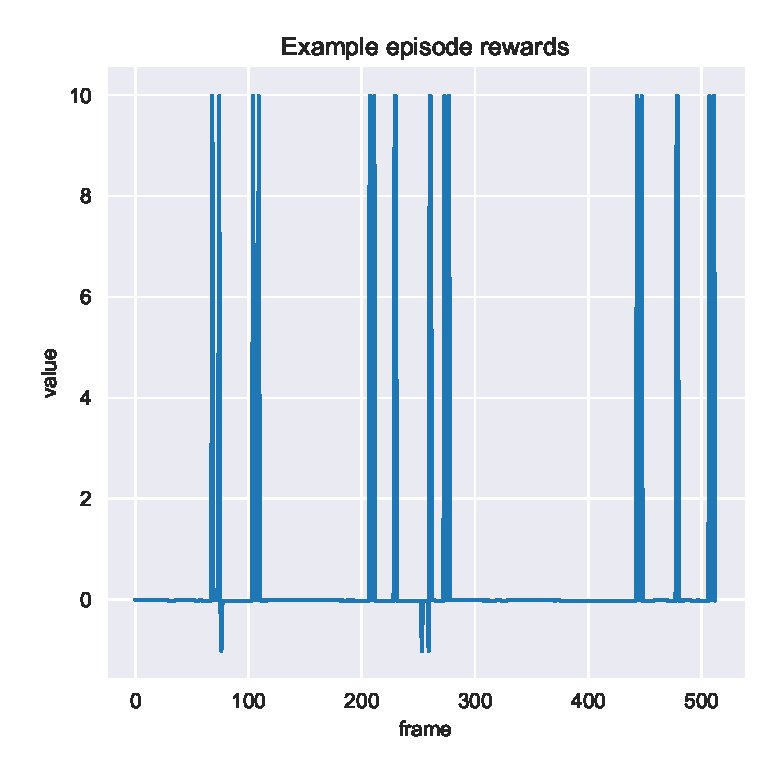
\includegraphics[scale=0.65]
    {./figures/example-episode-rewards}
    \caption{
        Example of instantaneous rewards for a single episode.
        The x-axis shows the frame, or step, when the reward was received, and the
        y-axis shows the reward.
        The high spikes are when the agent manages to eat food, while the low spikes
        are when the agent eats poison.
        Very slight dips can be seen as well, which are when the agent applies thrust.
    }
    \label{fig:example-episode-rewards}
\end{figure}

With this in mind, we developed two different types of memory: standard memory and
reward prioritized memory.

\subsubsection{Standard Memory}
Standard memory simply keeps track of the current state, actions, rewards, and next
states.
It can be sampled to return one or more record, which can then be used to train the
agent.

\subsubsection{Reward Prioritized Memory}
Reward prioritized memory is a special type of memory that, as with standard memory,
keeps track of the current state, actions, rewards, and next states.
However, it uses a simple algorithm to determine which records are more important/rare
than others and is more likely to return those memories when sampled.

The algorithm used to determine the rarity of a memory is simple.
A mean reward of 0 and a standard deviation of 0 are initialized.
Whenever a record is added to the memory buffer, the mean reward is updated as well as
the standard deviation.
When the memory is sampled, the z-score for each record is calculated and serves as
the record's weight.
Once all z-scores are calculated, the weights are used to randomly select samples
from the buffer.

The hope behind this structure was to emphasize those rare rewards and punishments in
an effort to accelerate learning and guide the agent towards the observations that
will most benefit the agent.

\subsection{Analysis Methods}\label{subsec:analysis-methods}
Analyses for this study were primarily based on total episode reward and the time it
took for an agent to settle.
Graphs were generated throughout training to monitor an agent's progress.
Whereas Waterworld each run is starts with random variables, some smoothing will then
be applied to these graphs to focus on general trends.

We will focus on four different analyses: Agent Type, Memory Type, Architecture, and
CPT\@.
The Agent Type portion will focus on the performance of different agents, as 
described in \autoref{subsec:training-algorithms}.
Likewise, Memory Type will focus on Reward Prioritized Memory vs Normal Memory, as 
described in \autoref{subsec:memory}, and Architecture will focus on Standard Networks
vs Distance Networks.
Whereas Waterworld has a time component, the Architecture section will also 
experiment with these networks with LSTM layers.
Finally, CPT will compare a DDPG Distance actor against a DDPG Distance actor trained
using a policy generated by \hyperref[subsubsec:cpt]{CPT}.

Agents with each combination of agent type, memory type, and architecture will be run
for the same number of iterations.
Afterwords, groupings will be made according to the analysis, and averages of rewards
and losses calculated.
Afterwards, graphs will be made to determine what difference, if any, there is for
each group.

% TODO: come back to this after finishing the results section.
